\chapter{Vergleich der Browser}
\label{chapter:vergleich-der-browser}

In diesem Kapitel werden die untersuchten Browser hinsichtlich der in Kapitel X identifizierten hinterlassenen PB Artefakte verglichen.

\subsection*{Common Locations}
Bei keinem Browser konnten PB Artefakte über die Analyse der Datei-Schreiboperationen in den Process Monitor Logfiles gefunden werden.
Ebenso konnten durch die genaue Untersuchung der Entwicklung der SQLite-Datenbänke aller Browser keine PB Artefakte identifiziert werden 
Somit sind die Common Locations aller Browser während der gesamten Versuchsdurchführung frei von PB Artefakten

\subsection*{Registry}
Bei Betrachtung der Registry als Common Locations wurden keine PB Artefakte in den Registry-Key bzw. -Values der Registry-Schreiboperationen der Process Monitor Logfiles gefunden.
Unter Betrachtung der Registry als Uncommon Locations konnten weder in System- noch User-Hives PB Artefakte gefunden werden.
Somit befinden sich bei jedem Browser auch in der Registry zu keinem Zeitpunkt PB Artefakte.



\subsection*{Uncommon Locations}
Weder über Autopsy Stichwortsuche noch in den automatisch von Autopsy kategorisierten Dateien konnten für keinen Browser PB Artefakte identifiziert werden.
%evtl. unterschiedlich Kategorisierte Dateien hervorheben

Einzig über die Untersuchung der Arbeitsspeicherabbilder mit Volatility konnten PB Artefakte zu unterschiedlichen Zeitpunkten der Versuchsdurchführung identifiziert werden. 
Wie in Abbildung \ref{chart:all-browsers-ram-summary} dargestellt, konnten in keinem der Browser im ersten RAM-Dump PB Artefakte gefunden werden. Somit befand sich vor dem Browsing Szenario kein PB Artefakt im Arbeitsspeicher der Browser.
\begin{table}[h!]
	\resizebox{\linewidth}{!}{
	\begin{tabular}{r}
		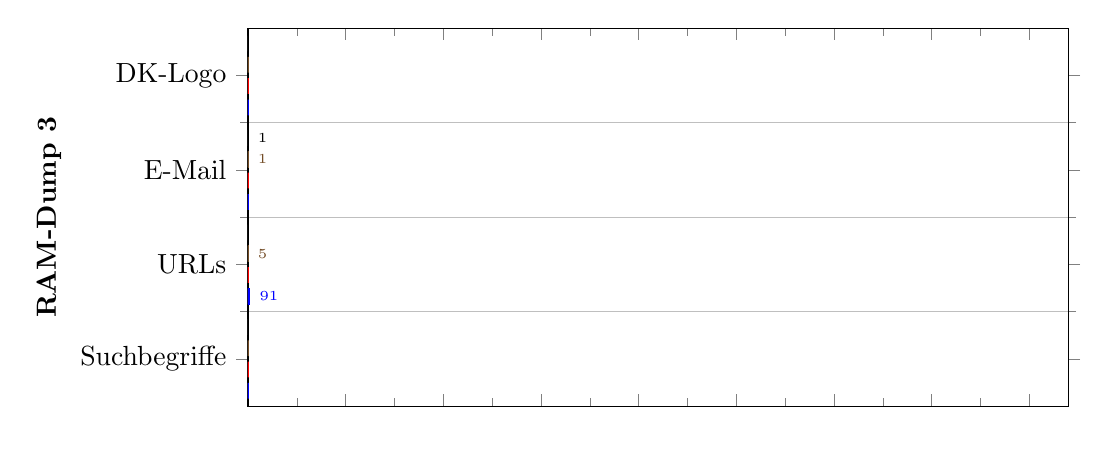
\begin{tikzpicture}
			\begin{axis}[
			xbar,
			width=12cm, 
			height=3cm, 
			ylabel style={align=center}, ylabel=\textbf{RAM-Dump 3},
			y=1.2cm,
			symbolic y coords={Suchbegriffe, URLs, E-Mail, DK-Logo},
			ytick=data,
			xticklabels={,,},
            xmin = 0,
            xmax = 42000,
			nodes near coords, 
			nodes near coords align={horizontal},
			nodes near coords style={font=\tiny},
   			nodes near coords={\pgfmathfloatifflags{\pgfplotspointmeta}{0}{}{\pgfmathprintnumber{\pgfplotspointmeta}}},
			bar width=.2cm,
			enlarge y limits={abs=3*\pgfplotbarwidth},
			scaled x ticks=false,
    		yminorgrids = true,minor tick num=1,
			legend style={
				at={(0.5,-0.1)},
				anchor=north
			},
			legend columns=4
			]
				\addplot coordinates {
				(0,Suchbegriffe) (91,URLs) (0,E-Mail) (0,DK-Logo)
				};
				\addplot coordinates {
				(0,Suchbegriffe) (0,URLs) (0,E-Mail) (0,DK-Logo)
				};
				\addplot coordinates {
				(0,Suchbegriffe) (5,URLs) (1,E-Mail) (0,DK-Logo)
				};
				\addplot coordinates {
				(0,Suchbegriffe) (0,URLs) (1,E-Mail) (0,DK-Logo)
				};
			\end{axis}
%			\legend{Firefox, Tor, Chrome, Brave}
		\end{tikzpicture}
		\\[-7pt]
		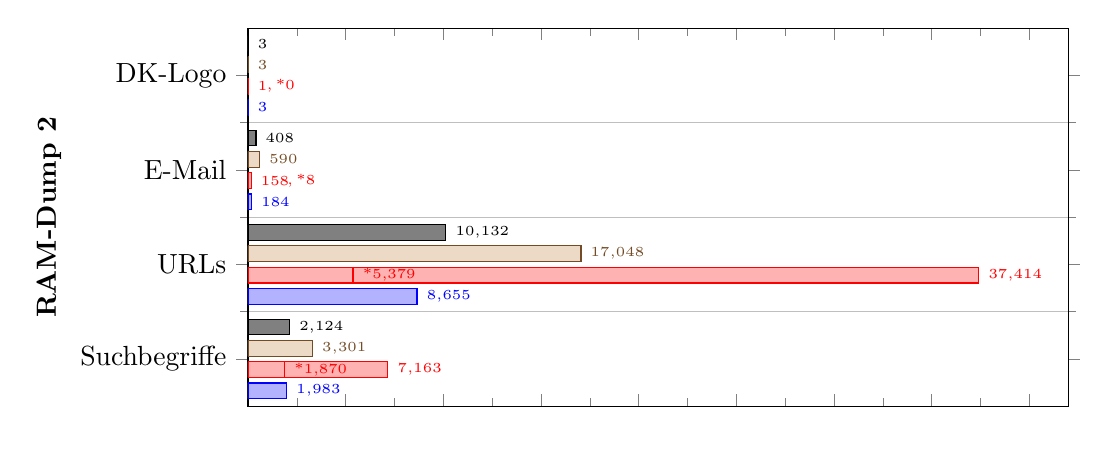
\begin{tikzpicture}
			\begin{axis}[
			xbar,
			width=12cm, 
			height=3cm, 
			ylabel style={align=center}, ylabel=\textbf{RAM-Dump 2},
			y=1.2cm,
%			symbolic y coords={Suchbegriffe, URLs, E-Mail, DK-Logo},
			ytick = {1,...,4},
			yticklabels={Suchbegriffe, URLs, E-Mail, DK-Logo},
			ytick=data,
			xticklabels={,,},
            xmin = 0,
            xmax = 42000,
			nodes near coords, 
			nodes near coords align={horizontal},
			nodes near coords style={font=\tiny},
   			nodes near coords={\pgfmathfloatifflags{\pgfplotspointmeta}{0}{}{\pgfmathprintnumber{\pgfplotspointmeta}}},
			bar width=.2cm,
			enlarge y limits={abs=3*\pgfplotbarwidth},
			scaled x ticks=false,
    		yminorgrids = true,minor tick num=1,
			legend style={
				at={(0.5,-0.1)},
				anchor=north
			},
			legend columns=4
			]
				\path  [red,line width=0pt] (axis cs: 500,3.977) -- (axis cs: 500,3.8)
				node[pos = 0.5,right] {\tiny,$\,$*0};
				\addplot coordinates {
				(1983,1) (8655,2) (184,3) (3,4)
				};
				\path  [red,line width=0pt] (axis cs: 1550,2.977) -- (axis cs: 1550,2.8)
				node[pos = 0.5,right] {\tiny,$\,$*8};
				\addplot coordinates {
				(7163,1) (37414,2) (158,3) (1,4)
				};
				\draw [red,line width=0.5pt] (axis cs: 5379,1.977) -- (axis cs: 5379,1.8)
				node[pos = 0.5,right] {\tiny*5,379};
				\addplot coordinates {
				(3301,1) (17048,2) (590,3) (3,4)
				};
				\draw [red,line width=0.5pt] (axis cs: 1870,0.977) -- (axis cs: 1870,0.8)
				node[pos = 0.5,right] {\tiny*1,870};
				\addplot coordinates {
				(2124,1) (10132,2) (408,3) (3,4)
				};
			\end{axis}
%			\legend{Firefox, Tor, Chrome, Brave}
		\end{tikzpicture}
		\\[-7pt]
		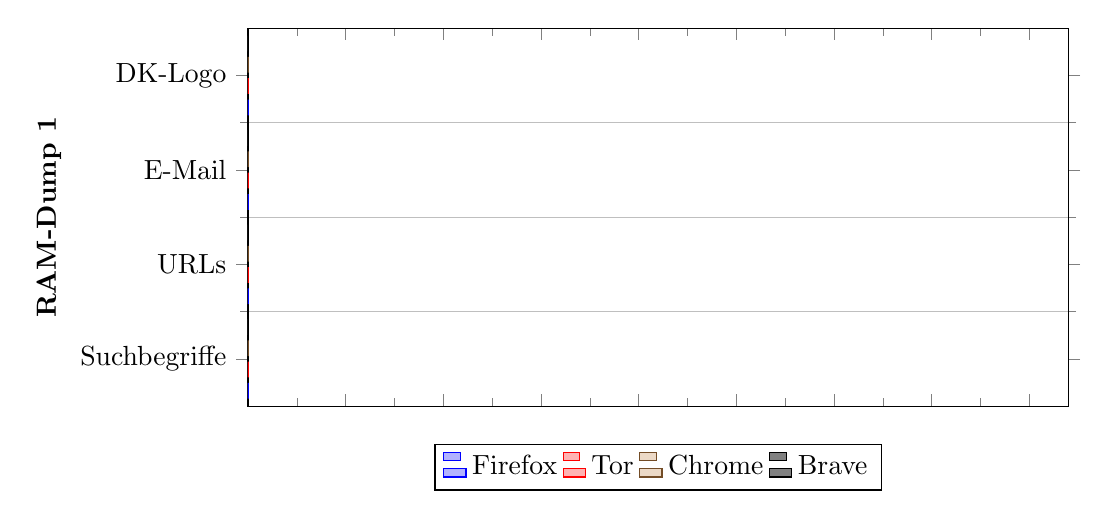
\begin{tikzpicture}
			\begin{axis}[
			xbar,
			width=12cm, 
			height=3cm, 
			ylabel style={align=center}, ylabel=\textbf{RAM-Dump 1},
			y=1.2cm,
%			symbolic y coords={Suchbegriffe, URLs, E-Mail, DK-Logo},
			ytick = {1,...,4},
			yticklabels={Suchbegriffe, URLs, E-Mail, DK-Logo},
%			ytick=data,
			xticklabels={,,},
            xmin = 0,
            xmax = 42000,
			nodes near coords, 
			nodes near coords align={horizontal},
			nodes near coords style={font=\tiny},
   			nodes near coords={\pgfmathfloatifflags{\pgfplotspointmeta}{0}{}{\pgfmathprintnumber{\pgfplotspointmeta}}},
			bar width=.2cm,
			enlarge y limits={abs=3*\pgfplotbarwidth},
			scaled x ticks=false,
    		yminorgrids = true,minor tick num=1,
			legend style={
				at={(0.5,-0.1)},
				anchor=north
			},
			legend columns=4
			]
				\addplot coordinates {
				(0,1) (0,2) (0,3) (0,4)
				};
				\addplot coordinates {
				(0,1) (0,2) (0,3) (0,4)
				};
				\addplot coordinates {
				(0,1) (0,2) (0,3) (0,4)
				};
				\addplot coordinates {
				(0,1) (0,2) (0,3) (0,4)
				};
			\legend{Firefox, Tor, Chrome, Brave}
			\end{axis}
		\end{tikzpicture}	
	\end{tabular}
	}
	\caption{Zusammenfassung gefundener Artefakte im RAM der Browser}
	\label{chart:all-browsers-ram-summary}
\end{table}

\paragraph*{Firefox vs Tor}
%> RAM-Dump 2: 
Tor hinterlässt nach dem Browsing Szenario mit geöffnetem Browser (RAM-Dump 2) mehr URL-Artefake und Suchbegriffe im RAM als Firefox. 
Sowohl Tor als auch Firefox hinterlassen zu diesem Zeitpunkt das Gmail-Passwort als Klartext im RAM.
Dieser Wert reduziert sich jedoch deutlich nachdem Tor eine ``Neuer Identität`` zugewiesen wird. 
Wie anhand der mit * gekennzeichneten Werte in Abbildung \ref{chart:all-browsers-ram-summary} zu erkennen ist, befinden sich danach bei jeder Kategorie deutlich weniger Artefake im RAM von Tor als bei Firefox. 
Weitherin ist danach das Passwort nicht mehr als Klartext im RAM von Tor zu finden.
%> RAM-Dump 3:
Nach Schließen des Browsers (RAM-Dump 3) konnten bei Firefox noch 91 URLs im DNSCache gefunden werden. 
Tor hinterlässt keine Artefakte nach Schließen des Browsers.
%Gewinner:
%> RAM-Dump 2:
%	- Vor ``Neue Identität``: Firefox
%	- Nach ``Neuer Identität``: Tor 
%> RAM-Dump 3:
%	- Tor 
%Somit hinterlässt Tor sowohl nach dem Browsing Szenario mit ``Neuer Identität`` als auch mit geschlossenem Browser weniger PB Artefakte als Firefox.

\paragraph*{Chrome vs Brave}
> ... *** TODO: Christoph ***
=> Brave hinterlässt weniger Artefakte als Chrome

\paragraph*{Firefox vs Chrome}
%> In RAM-Dump 2: 
Firefox hinterlässt nach dem Browsing Szenario mit geöffnetem Browser (RAM-Dump 2) in jeder Kategorie gleich viele (DK-Logo) oder weniger (E-Mail, URLs, Suchbegriffe) Artefakte als Chrome.
Dabei werden bei Firefox durchschnittlich 2.529 Artefakte weniger gefunden als bei Chrome.
%> In Ram-Dump 3: 
Nach Schließen des Browsers hinterlässt Firefox mehr URLs als Chrome im RAM. Im RAM-Dump von Chrome wurde zusätzlich die Absender-Adresse gefunden.
%Gewinner:
%RAM-Dump 2:
%	- Firefox
%RAM-Dump 3: 
%	- URLs: Chrome
%	- E-Mail: Firefox

\paragraph*{Tor vs Brave}
Vor Zuweisung der ``Neuen Identität`` hinterlässt der Tor-Browser nach dem Browsing-Szenario deutlich mehr URL- und Suchbegriff-Artefakte als Brave. Insbesondere hinterlässt Tor zweimal das Passwort des Google-Accounts als Klartext im RAM.
Nach Zuweisung der ``Neuen Identiät`` des Tor-Browsers hinterlässt dieser im RAM-Dump 2 durchschnittlich 1315 Artefakte weniger als Brave.
Nach Schließen des Browsers (RAM-Dump 3) hinterlässt Tor kein Artefakt im RAM, Brave die Absender-Mail. 
%Gewinner:
%RAM-Dump 2:
%	- DK-Logo, E-Mail: Tor
%	- URLs, Suchbegriffe: Brave (Vor ``Neue Identität``), Tor (Nach ``Neuer Identität``) 
%RAM-Dump 3: Tor

\paragraph*{Quantitativer Vergleich aller Browser}
Um unter den vier untersuchten Browsern denjenigen mit den wenigsten PB Artefakten zu ermitteln, wird die sogenannte in Tabelle \ref{tab:gewinner-tabelle} gezeigte \textit{Gewinner-Tabelle} erstellt (TODO: Quelle).

\begin{table}[h!]
	\caption{Gewinner-Tabelle der vier untersuchten Browser}
	\label{tab:gewinner-tabelle}
	\centering
	\resizebox{\linewidth}{!}{
	\begin{tabular}{c|c|c|c|c|c}
	\cline{2-6}
	\multicolumn{1}{l|}{}                                                                                                    & \textbf{Suchbegriffe}                   & \textbf{URLs}                                       & \textbf{E-Mail}                                      & \textbf{DK-Logo}                    & \multicolumn{1}{c|}{\textbf{Gewinner pro RAM-Dump}}                \\ \hline
	\multicolumn{1}{|c|}{\textbf{RAM-Dump 1}}                                                                                & Unentschieden                           & Unentschieden                                       & Unentschieden                                        & Unentschieden                       & \multicolumn{1}{c|}{{\color[HTML]{FE0000} \textbf{Unentschieden}}} \\ \hline
	\multicolumn{1}{|c|}{\textbf{\begin{tabular}[c]{@{}c@{}}RAM-Dump 2\\ (ohne ``Neuer Identität``)\end{tabular}}}             & Firefox                                 & Firefox                                             & Brave\tablefootnote{Bemerkung zu Brave: Obwohl Firefox und der Tor-Browser weniger E-Mail Artefakte hinterlassen, wurde das Auffinden des Passworts als Klartext als so kritisch angesehen, dass Brave im zweiten RAM-Dump (ohne ``Neue Identität`` des Tor-Browser) als Bester Browser gewählt wurde.}                                               & Tor                                 & \multicolumn{1}{c|}{{\color[HTML]{FE0000} \textbf{Firefox}}}       \\ \hline
	\multicolumn{1}{|c|}{\textbf{\begin{tabular}[c]{@{}c@{}}RAM-Dump 2\\ (mit ``Neuer Identität``)\end{tabular}}}              & Tor                                     & Tor                                                 & Tor                                                  & Tor                                 & \multicolumn{1}{c|}{{\color[HTML]{FE0000} \textbf{Tor}}}           \\ \hline
	\multicolumn{1}{|c|}{\textbf{RAM-Dump 3}}                                                                                & Unentschieden                           & Tor, Brave                                          & Firefox, Tor                                         & Unentschieden                       & \multicolumn{1}{c|}{{\color[HTML]{FE0000} \textbf{Tor}}}           \\ \hline
	\multicolumn{1}{|c|}{\textbf{\begin{tabular}[c]{@{}c@{}}Gewinner pro Kategorie\\ (ohne ``Neuer Identität``)\end{tabular}}} & {\color[HTML]{FE0000} \textbf{Firefox}} & {\color[HTML]{FE0000} \textbf{Firefox, Tor, Brave}} & {\color[HTML]{FE0000} \textbf{Firefox, Tor, Brave$^{1}$}} & {\color[HTML]{FE0000} \textbf{Tor}} & \multicolumn{1}{l}{}                                               \\ \cline{1-5}
	\multicolumn{1}{|c|}{\textbf{\begin{tabular}[c]{@{}c@{}}Gewinner pro Kategorie\\ (mit``Neuer Identität``)\end{tabular}}}   & {\color[HTML]{FE0000} \textbf{Tor}}     & {\color[HTML]{FE0000} \textbf{Tor}}                 & {\color[HTML]{FE0000} \textbf{Tor}}                  & {\color[HTML]{FE0000} \textbf{Tor}} & \multicolumn{1}{l}{}                                               \\ \cline{1-5}
	\end{tabular}
	}
\end{table}

Dabei liegt der Fokus auf den Kategorien der PB-Artefakte: Die Anzahl gefundener Artefakte wird nur innerhalb einer Kategorie verglichen. Die Differenz der Anzahl gefundener PB Artefakte wird dabei nicht berücksichtigt. Es wird für jede RAM-Dump/Kategorie Kombination derjenige Browser mit den wenigsten PB Artefakten ermittelt. Per Mehrheitseinscheid ergeben sich daraus zwei Arten von \textit{Gewinnern}:
\begin{itemize}
\item \textbf{Gewinner pro RAM-Dump}: Browser, der innerhalb eines RAM-Dumps am häufigsten die wenigsten PB Artefakte einer Kategorie hinterlässt
\item \textbf{Gewinner pro Kategorie}: Browser, der innerhalb einer Kategorie am häufigsten die wenigsten PB-Artefakte in einem RAM-Dump hinterlässt.
\end{itemize}

Um ein differenziertes Ergebnis zu ermitteln, wird bei RAM-Dump 2 zusätzlich unterschieden, ob der Tor-Browser vor- oder nach der Zuweisung der ``Neuen Identität`` bewertet wird. 
Diese Unterscheidung findet ebenfalls bei den Gewinnern statt. Somit ergeben sich die in Tabelle \ref{tab:gewinner} ermittelten vier Gewinner:

\begin{table}[h!]
	\centering
	\caption{Ermittelte Gewinner gemäß Gewinner-Tabelle}
	\label{tab:gewinner}
	\resizebox{0.8\linewidth}{!}{
	\begin{tabular}{c|c|c|}
	\cline{2-3}
	\multicolumn{1}{l|}{}                                 & \textbf{Mit ``Neuer Identität``} & \textbf{Ohne ``Neuer Identität``} \\ \hline
	\multicolumn{1}{|c|}{\textbf{Gewinner pro RAM-Dump}}  & Tor                            & Firefox, Tor                    \\ \hline
	\multicolumn{1}{|c|}{\textbf{Gewinner pro Kategorie}} & Tor                            & Firefox, Tor                    \\ \hline
	\end{tabular}
	}
\end{table}

Unter Berücksichtigung der ``Neuen Identität`` ist der Tor-Browser sowohl der Gewinner pro RAM-Dump als auch pro Kategorie.
Ohne Berücksichtigung ist neben dem Tor-Browser auch Firefox Gewinner pro RAM-Dump und pro Kategorie. Somit ist gemäß Auswertung der Gewinner-Tabelle der Tor-Browser derjenige Browser mit den wenigsten PB Artefakten, gefolgt von Mozilla Firefox.











